\documentclass[tikz,border=8pt]{standalone}
\usepackage[T1]{fontenc}
\usepackage[utf8]{inputenc}
\usepackage{lmodern}
\usepackage{textcomp}
\usepackage{tikz}
\usetikzlibrary{arrows.meta,calc,positioning}

\begin{document}
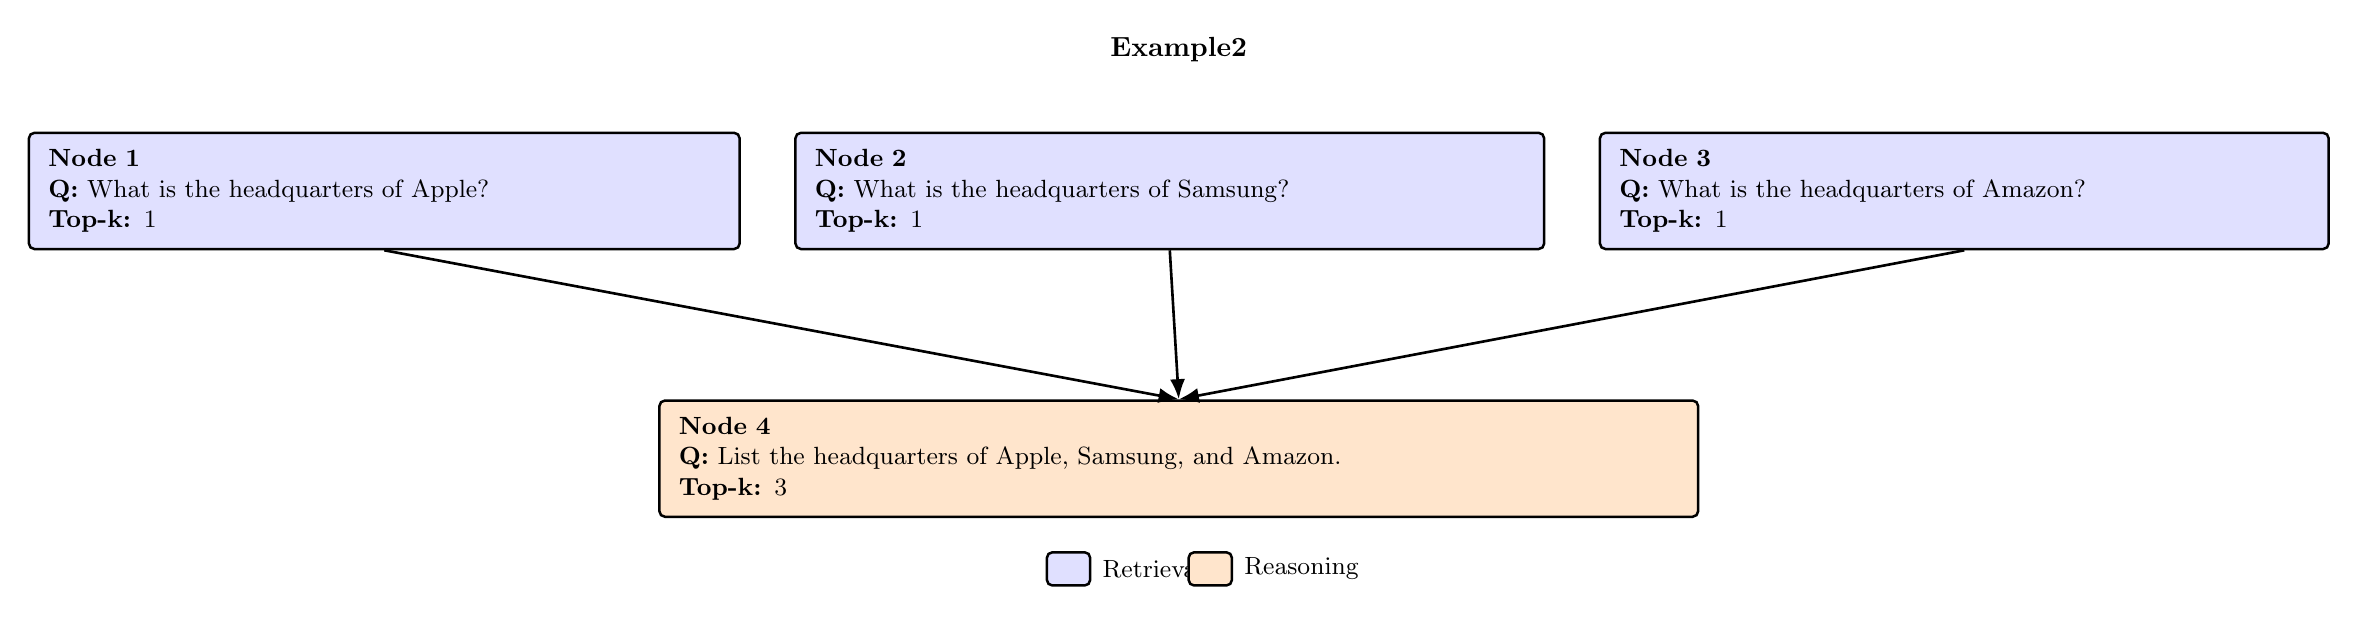
\begin{tikzpicture}[
  x=1cm,
  y=1cm,
  >=Latex,
  line width=0.9pt,
  every node/.style={font=\small},
  dagbox/.style={
    draw,
    rounded corners=2pt,
    align=left,
    inner xsep=7pt,
    inner ysep=6pt,
    minimum height=1.3cm,
  },
  dagbox retrieval/.style={dagbox, fill=blue!12},
  dagbox reasoning/.style={dagbox, fill=orange!20},
  dagarrow/.style={->, line width=0.95pt},
]
\node[font=\normalsize\bfseries] at (0,1.8) {Example2};
\node[dagbox retrieval, text width=3.36in] (N1) at (-10.090,0.000) {\textbf{Node 1} \\ \textbf{Q:} What is the headquarters of Apple? \\ \textbf{Top-k:} 1};
\node[dagbox retrieval, text width=3.55in] (N2) at (-0.114,0.000) {\textbf{Node 2} \\ \textbf{Q:} What is the headquarters of Samsung? \\ \textbf{Top-k:} 1};
\node[dagbox retrieval, text width=3.45in] (N3) at (9.976,0.000) {\textbf{Node 3} \\ \textbf{Q:} What is the headquarters of Amazon? \\ \textbf{Top-k:} 1};
\node[dagbox reasoning, text width=5.00in] (N4) at (0.000,-3.400) {\textbf{Node 4} \\ \textbf{Q:} List the headquarters of Apple, Samsung, and Amazon. \\ \textbf{Top-k:} 3};
\draw[dagarrow] (N1.south) -- (N4.north);
\draw[dagarrow] (N2.south) -- (N4.north);
\draw[dagarrow] (N3.south) -- (N4.north);
\node[dagbox retrieval, minimum width=0.55cm, minimum height=0.35cm] at (-1.4,-4.80) {};
\node[anchor=west, font=\small] at (-1.1,-4.80) {Retrieval};
\node[dagbox reasoning, minimum width=0.55cm, minimum height=0.35cm] at (0.4,-4.80) {};
\node[anchor=west, font=\small] at (0.7,-4.80) {Reasoning};
\end{tikzpicture}
\end{document}